% 【拆分生成】 questions.tex —— 2025 年·全国 2 卷 · 题目内容片段（无答案）
% 【拆分生成】 由 tools/split_project.py 自合并书 papers/2025_g2.tex 包裹 question 环境生成，勿手改
% 由 tools/md2tex.py 自 2025_数学真题_全国2_试题.md 生成，勿手改（改源 MD 后重跑）


\begin{gknotice}
\textbf{适用省份}：辽宁、重庆、海南、吉林、黑龙江、山西、云南、广西、甘肃、贵州、新疆、四川、内蒙古、陕西、青海、宁夏、西藏

\textbf{来源说明}：试题原文取自 deekur/gaokaomath（commit \texttt{34c13a6}，CC BY 4.0）之 \texttt{2025全国2} PDF；本库配套解析为编者独立推导，\textbf{非官方标准答案}。
\end{gknotice}

\par\medskip

\gkpart{一、单选题}

\begin{gktip}
本题共 8 小题，每小题 5 分，共 40 分。在每小题给出的四个选项中，只有一项是符合题目要求的。
\end{gktip}

\begin{question}
\gkti{1}样本数据 $2,8,14,16,20$ 的平均数为（　　）

\begin{gkopts}(4)
\task A．$8$
\task B．$9$
\task C．$12$
\task D．$18$
\end{gkopts}

\end{question}
\begin{question}
\gkti{2}已知 $z=1+\mathrm{i}$，则 $\dfrac{1}{z-1}=$（　　）

\begin{gkopts}(4)
\task A．$-\mathrm{i}$
\task B．$\mathrm{i}$
\task C．$-1$
\task D．$1$
\end{gkopts}

\end{question}
\begin{question}
\gkti{3}已知集合 $A=\{-4,0,1,2,8\}$，$B=\left\{x\mid x^3=x\right\}$，则 $A\cap B=$（　　）

\begin{gkopts}(4)
\task A．$\{0,1,2\}$
\task B．$\{1,2,8\}$
\task C．$\{2,8\}$
\task D．$\{0,1\}$
\end{gkopts}

\end{question}
\begin{question}
\gkti{4}不等式 $\dfrac{x-4}{x-1}\ge 2$ 的解集是（　　）

\begin{gkopts}(2)
\task A．$\{x\mid -2\le x\le 1\}$
\task B．$\{x\mid x\le -2\}$
\task C．$\{x\mid -2\le x<1\}$
\task D．$\{x\mid x>1\}$
\end{gkopts}

\end{question}
\begin{question}
\gkti{5}在 $\triangle ABC$ 中，$BC=2$，$AC=1+\sqrt3$，$AB=\sqrt6$，则 $A=$（　　）

\begin{gkopts}(4)
\task A．$45^\circ$
\task B．$60^\circ$
\task C．$120^\circ$
\task D．$135^\circ$
\end{gkopts}

\end{question}
\begin{question}
\gkti{6}设抛物线 $C:y^2=2px\ (p>0)$ 的焦点为 $F$，点 $A$ 在 $C$ 上，过 $A$ 作 $C$ 的准线的垂线，垂足为 $B$．若直线 $BF$ 的方程为 $y=-2x+2$，则 $|AF|=$（　　）

\begin{gkopts}(4)
\task A．$3$
\task B．$4$
\task C．$5$
\task D．$6$
\end{gkopts}

\end{question}
\begin{question}
\gkti{7}记 $S_n$ 为等差数列 $\{a_n\}$ 的前 $n$ 项和．若 $S_3=6$，$S_5=-5$，则 $S_6=$（　　）

\begin{gkopts}(4)
\task A．$-20$
\task B．$-15$
\task C．$-10$
\task D．$-5$
\end{gkopts}

\end{question}
\begin{question}
\gkti{8}已知 $0<\alpha<\pi$，$\cos\dfrac{\alpha}{2}=\dfrac{\sqrt5}{5}$，则 $\sin\left(\alpha-\dfrac{\pi}{4}\right)=$（　　）

\begin{gkopts}(2)
\task A．$\dfrac{\sqrt2}{10}$
\task B．$\dfrac{\sqrt2}{5}$
\task C．$\dfrac{3\sqrt2}{10}$
\task D．$\dfrac{7\sqrt2}{10}$
\end{gkopts}

\par\medskip

\end{question}
\gkpart{二、多选题}

\begin{gktip}
本题共 3 小题，每小题 6 分，共 18 分。在每小题给出的选项中，有多项符合题目要求。全部选对的得 6 分，部分选对的得部分分，有选错的得 0 分。
\end{gktip}

\begin{question}
\gkti{9}记 $S_n$ 为等比数列 $\{a_n\}$ 的前 $n$ 项和，$q$ 为 $\{a_n\}$ 的公比，$q>0$．若 $S_3=7$，$a_3=1$，则（　　）

\begin{gkopts}(4)
\task A．$q=\dfrac12$
\task B．$a_5=\dfrac19$
\task C．$S_5=8$
\task D．$a_n+S_n=8$
\end{gkopts}

\end{question}
\begin{question}
\gkti{10}已知 $f(x)$ 是定义在 $\mathbf{R}$ 上的奇函数，且当 $x>0$ 时，$f(x)=\left(x^2-3\right)\mathrm{e}^{x}+2$，则（　　）

\begin{gkopts}(1)
\task A．$f(0)=0$
\task B．当 $x<0$ 时，$f(x)=-\left(x^2-3\right)\mathrm{e}^{-x}-2$
\task C．$f(x)\ge 2$ 当且仅当 $x\ge\sqrt3$
\task D．$x=-1$ 是 $f(x)$ 的极大值点
\end{gkopts}

\end{question}
\begin{question}
\gkti{11}双曲线 $C:\dfrac{x^2}{a^2}-\dfrac{y^2}{b^2}=1\ (a>0,\ b>0)$ 的左、右焦点分别为 $F_1$，$F_2$，左、右顶点分别为 $A_1$，$A_2$，以 $F_1F_2$ 为直径的圆与 $C$ 的一条渐近线交于 $M$，$N$ 两点，且 $\angle NA_1M=\dfrac{5\pi}{6}$，则（　　）

\begin{gkopts}(1)
\task A．$\angle A_1MA_2=\dfrac{\pi}{6}$
\task B．$|MA_1|=2|MA_2|$
\task C．$C$ 的离心率为 $\sqrt{13}$
\task D．当 $a=\sqrt2$ 时，四边形 $NA_1MA_2$ 的面积为 $8\sqrt3$
\end{gkopts}

\par\medskip

\end{question}
\gkpart{三、填空题}

\begin{gktip}
本题共 3 小题，每小题 5 分，共 15 分。
\end{gktip}

\begin{question}
\gkti{12}已知平面向量 $\boldsymbol{a}=(x,1)$，$\boldsymbol{b}=(x-1,2x)$，若 $\boldsymbol{a}\perp(\boldsymbol{a}-\boldsymbol{b})$，则 $|\boldsymbol{a}|=$ \gkblank{}．

\end{question}
\begin{question}
\gkti{13}若 $x=2$ 是函数 $f(x)=(x-1)(x-2)(x-a)$ 的极值点，则 $f(0)=$ \gkblank{}．

\end{question}
\begin{question}
\gkti{14}一个底面半径为 $4\ \mathrm{cm}$，高为 $9\ \mathrm{cm}$ 的封闭圆柱形容器（容器壁厚度忽略不计）内有两个半径相等的铁球，则铁球半径的最大值为 \gkblank{} $\mathrm{cm}$．

\par\medskip

\end{question}
\gkpart{四、解答题}

\begin{gktip}
本题共 5 小题，共 77 分。解答应写出文字说明、证明过程或演算步骤。
\end{gktip}

\begin{question}
\gkti{15}\textbf{（13 分）} 已知函数 $f(x)=\cos(2x+\varphi)\ (0\le\varphi<\pi)$，$f(0)=\dfrac12$．

  (1) 求 $\varphi$；

  (2) 设函数 $g(x)=f(x)+f\left(x-\dfrac{\pi}{6}\right)$，求 $g(x)$ 的值域和单调区间．

\end{question}
\begin{question}
\gkti{16}\textbf{（15 分）} 已知椭圆 $C:\dfrac{x^2}{a^2}+\dfrac{y^2}{b^2}=1\ (a>b>0)$ 的离心率为 $\dfrac{\sqrt2}{2}$，长轴长为 $4$．

  (1) 求 $C$ 的方程；

  (2) 过点 $(0,-2)$ 的直线 $l$ 与 $C$ 交于 $A$，$B$ 两点，$O$ 为坐标原点．若 $\triangle OAB$ 的面积为 $\sqrt2$，求 $|AB|$．

\end{question}
\begin{question}
\gkti{17}\textbf{（15 分）} 如图，在四边形 $ABCD$ 中，$AB\parallel CD$，$\angle DAB=90^\circ$，$F$ 为 $CD$ 的中点，点 $E$ 在 $AB$ 上，$EF\parallel AD$，$AB=3AD$，$CD=2AD$．将四边形 $EFDA$ 沿 $EF$ 翻折至四边形 $EFD'A'$，使得面 $EFD'A'$ 与面 $EFCB$ 所成的二面角为 $60^\circ$．

\begin{center}% 2025 全国 2 卷 17：正方形沿 EF 翻折后的四棱锥体（A、D 翻折到 A'、D'）
% 立体坐标 E(0,0,0)、B(2,0,0)、F(0,1,0)、C(1,1,0)、A'(1/2,0,√3/2)、D'(1/2,1,√3/2)，
% 翻折前的位置 A(-1,0,0)、D(-1,1,0) 以虚影正方形 AEFD 保留，示折痕 EF 的来源。
% 画布投影：(x,y,z) -> x·(1,0) + y·(0.35,0.45) + z·(0,1)。
% 虚线：被遮挡的 EF、FC、CB、FD'、D'C，以及翻折前的虚影边 AE、AD、DF。
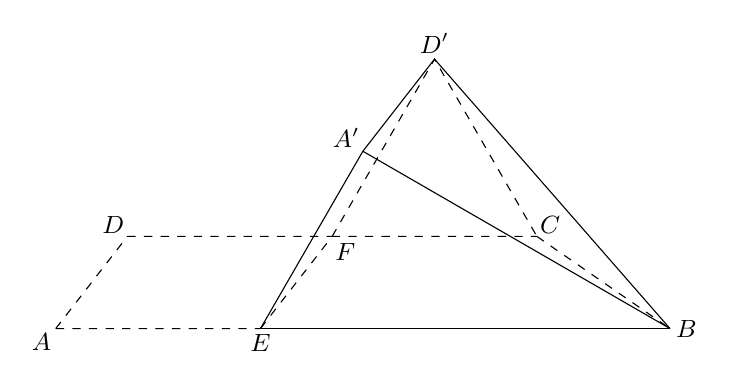
\begin{tikzpicture}[scale=2.6, font=\small]
  \coordinate (E)  at (0,0);
  \coordinate (B)  at (2,0);
  \coordinate (F)  at (0.35,0.45);
  \coordinate (C)  at (1.35,0.45);
  \coordinate (Ap) at (0.5,0.866);
  \coordinate (Dp) at (0.85,1.316);
  \coordinate (A)  at (-1,0);
  \coordinate (D)  at (-0.65,0.45);
  % 可见实线
  \draw (E) -- (B);
  \draw (E) -- (Ap) -- (Dp) -- (B);
  \draw (Ap) -- (B);
  \draw[dashed] (C) -- (B);
  % 被遮挡
  \draw[dashed] (E) -- (F) -- (C);
  \draw[dashed] (F) -- (Dp) -- (C);
  % 翻折前的虚影正方形 AEFD
  \draw[dashed] (A) -- (E)  (A) -- (D)  (D) -- (F);
  \node[below left,  inner sep=1.5pt] at (A)  {$A$};
  \node[above left,  inner sep=1pt]   at (D)  {$D$};
  \node[below,       inner sep=2pt]   at (E)  {$E$};
  \node[below right, inner sep=1pt, yshift=-1.5pt] at (F) {$F$};
  \node[above right, inner sep=1pt]   at (C)  {$C$};
  \node[right,       inner sep=2pt]   at (B)  {$B$};
  \node[above left,  inner sep=1pt]   at (Ap) {$A'$};
  \node[above,       inner sep=2pt]   at (Dp) {$D'$};
\end{tikzpicture}
\end{center}

  (1) 证明：$A'B\parallel$ 平面 $CD'F$；

  (2) 求面 $BCD'$ 与面 $EFD'A'$ 所成的二面角的正弦值．

\end{question}
\begin{question}
\gkti{18}\textbf{（17 分）} 已知函数 $f(x)=\ln(1+x)-x+\dfrac12x^2-kx^3$，其中 $0<k<\dfrac13$．

  (1) 证明：$f(x)$ 在区间 $(0,+\infty)$ 存在唯一的极值点和唯一的零点；

  (2) 设 $x_1$，$x_2$ 分别为 $f(x)$ 在区间 $(0,+\infty)$ 的极值点和零点．

  　① 设函数 $g(t)=f(x_1+t)-f(x_1-t)$．证明：$g(t)$ 在区间 $(0,x_1)$ 单调递减；

  　② 比较 $2x_1$ 与 $x_2$ 的大小，并证明你的结论．

\end{question}
\begin{question}
\gkti{19}\textbf{（17 分）} 甲、乙两人进行乒乓球练习，每个球胜者得 $1$ 分，负者得 $0$ 分．设每个球甲胜的概率为 $p\ \left(\dfrac12<p<1\right)$，乙胜的概率为 $q$，$p+q=1$，且各球的胜负相互独立．对正整数 $k\ge 2$，记 $p_k$ 为打完 $k$ 个球后甲比乙至少多得 $2$ 分的概率，$q_k$ 为打完 $k$ 个球后乙比甲至少多得 $2$ 分的概率．

  (1) 求 $p_3$，$p_4$（用 $p$ 表示）；

  (2) 若 $\dfrac{p_4-p_3}{q_4-q_3}=4$，求 $p$；

  (3) 证明：对任意正整数 $m$，$p_{2m+1}-q_{2m+1}<p_{2m}-q_{2m}<p_{2m+2}-q_{2m+2}$．

\par\medskip

\begin{gktip}
\textbf{试题来源}：deekur/gaokaomath（commit \texttt{34c13a6}，CC BY 4.0）之 \texttt{2025全国2} PDF。
\end{gktip}

\end{question}